
\begin{figure}
\centering
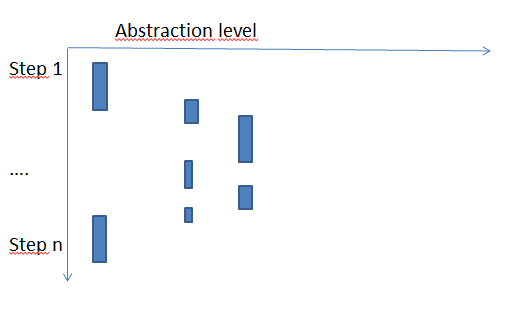
\includegraphics{Bilder/Rule1Abstraction.png}
\caption[Diagramm showing the result when applying rule 1]{Diagramm showing the result when applying rule 1}
\label{picture:rule1abstraction}
\end{figure}


\begin{figure}
\centering
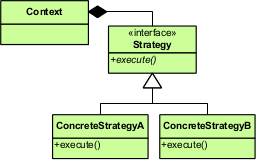
\includegraphics{Bilder/StrategyPattern.png}
\caption[\acf{UML} diagram of the strategy pattern]{\acf{UML} diagram of the strategy pattern}
\label{picture:strategypattern}
\end{figure}


\begin{figure}
\centering
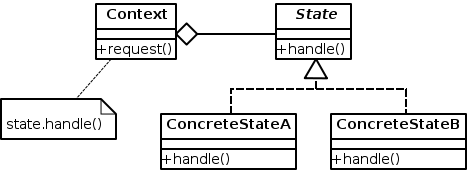
\includegraphics{Bilder/StatePattern.png}
\caption[\acf{UML} diagram of the state pattern]{\acf{UML} diagram of the state pattern}
\label{picture:statepattern}
\end{figure}

\begin{figure}
\centering
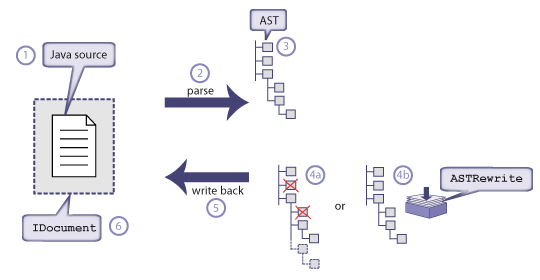
\includegraphics{Bilder/workflowAST.png}
\caption[Workflow of the eclipse frameworks that allows to read and modify the \acf{AST}]{Workflow of the eclipse frameworks that allows to read and modify the \acf{AST}}
\label{picture:workflowast}
\end{figure}

\begin{figure}
\centering
\includegraphics{Bilder/violationtable.png}
\caption[Table showing all the necessary violations in a table]{Table showing all the necessary violations in a table}
\label{picture:violationtable}
\end{figure}
